\chapter{Development}

The result of this research was the development of |miq|, a package manager and
build system for Linux.

miq is a single-file executable that handles the full lifecycle of the build
process of the packages it manages. This stages include:

\begin{enumerate}
    \item Evaluating the expressions that describe packages
    \item Calculating the dependency graph
    \item Fetching the necessary source code
    \item Performing the described build process
    \item Handling the storage and tracking of the installed packages
\end{enumerate}

Therefore, the following sections will all the components that make up miq, and
their interactions.

\section{High level overview}

The development of miq aimed for a modular design, such that
each component didn't have much coupling with the others.
This allows for easy refactoring of parts of the source
code, while leaving the rest of the system untouched. As
such the components of miq can be layed out in figure
\ref{fig:miq-components} .

\begin{figure}
    \centerfloat
    % 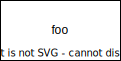
\includegraphics{assets/overview.png}
    \includesvg[width = 450pt]{assets/overview.svg}
    \caption{Overview of the subsystems of miq}
    \label{fig:miq-components}
\end{figure}

Miq is presented as a pipeline of stages, where each
subsystem transform the input data to achieve a desired
state. This design is inspired by other package managers,
which present a similar structure of stages. The main
difference, is that miq works on static package definitions
layed out in a file, which describe the desired state of the
system. In contrast to other package managers, like |apt|,
where the final state of the system is a succession of
commands executed in the shell.

On of the main differences of miq to other package managers,
is how the files are layed out in the filesystem. This is
because each package is given a unique identifier, which in
turns is used for the directory where the package will be
located. This identifier is also unique between different
versions of the same package. And not only that, but it also
encodes the recipe used to build the package itself, and all
of its parents.

To accomplish the tagging of each package with an unique
identifier, a flow of data from package input to package is
visualized on figure \ref{fig:hash}. From a |PackageInput|,
a unique hash is generated, that is the result from hashing
all the fields of the struct. Finally, the hash (an unsigned
32-bit integer) is encoded into text, to form the name of
the package. For this application, the algorithm used is the
\textit{Fowler-Noll-V}o hash function, which is implemented
in the |fnv| create \cite{FnvRust} . This hash function is
not cryptographically secure, but this was not one of the
design requirements of miq (and can be swapped out for any
other hashing algorithm as needed, as long as it conforms to
the |Hash| trait in Rust).



\begin{minted}{rust}
#[derive(Hash)]
struct PackageInput {
    name: String,
    version: Option<String>,
    script: MetaTextInput,
    deps: Option<Vec<Unit>>,
    env: Option<BTreeMap<String, MetaTextInput>>,
}
\end{minted}

\begin{figure}
    \centerfloat
    \includesvg[width = 300pt]{assets/hash.svg}
    \caption{Overview of the hashing algorithm}
    \label{fig:hash}
\end{figure}

The implications of this design is that any package gets a
different place on the filesystem, which is derived from
everything that defines the package itself - its build
script and its dependencies, which in turn are also hashed
by the same rules. The advantage of this design, is that
every package has its dependencies perfectly defined,
instead of relying on automatic detection. Let's say that
package |foo| depends of package |bar|. On a conventional
package manager, if |bar| is changed in any form (for
example, updated), then |foo| is usually not modified. But
in essence, now |foo|, if we consider it as a whole, that is
its whole dependency tree, it has changed. This poses a big
issue for the reproducibility of an operating system. Is
|foo| the same if we swapped |bar| for a different version?
Or if we swapped one of |bar|'s dependencies? (Figure
\ref{fig:depswap}) In miq, it is clear that the packages are
no longer the same, as the hashes of its entire dependency
tree has changed, and therefore the name of the output
package. This means that a package "foo" does not really
exist in miq, but rather a package "foo" with a specific hash.

\begin{figure}
    \centerfloat
    \includesvg[width = 200pt]{assets/depswap.svg}
    \caption{Change of dependencies for a package for a conventional package manager}
    \label{fig:depswap}
\end{figure}

% insert depswap-miq.svg
\begin{figure}
    \centerfloat
    \includesvg[width = 200pt]{assets/depswap_miq.svg}
    \caption{Change of dependencies for a package for miq}
    \label{fig:depswap_miq}
\end{figure}

\subsection{Graph based dependencies}

\subsection{Immutability}

\subsection{Stages}

\subsection{Atomic changes}

\subsection{ELF format}


\section{Builder}

\section{Graph evaluator}

\section{Lua evaluator}

\section{Other components}

